
%\documentclass[journal=jacsat, manuscript=article]{achemso}

\documentclass[varwidth, border={1pt 1pt 1pt 1pt}]{standalone}
 % left right bottom top
 \usepackage{graphicx}
%\usepackage{subcaption}
\graphicspath{/}
\usepackage{amsmath}
\usepackage{subfig}
\usepackage {tikz}
\usepackage{pgfplots}
\pgfplotsset{compat=1.12}
\usepackage{nomencl}
\usepackage{lineno}
\usepackage[toc,page]{appendix}
%\linenumbers %reenable before submission
%\makenomenclature
\usepackage{comment}
%\usepackage[margin=0.1in]{geometry}






\begin{document}
\newpage
\begin{figure}
    \centering
    
	\subfloat[Narrow, 1:1 ion]{
		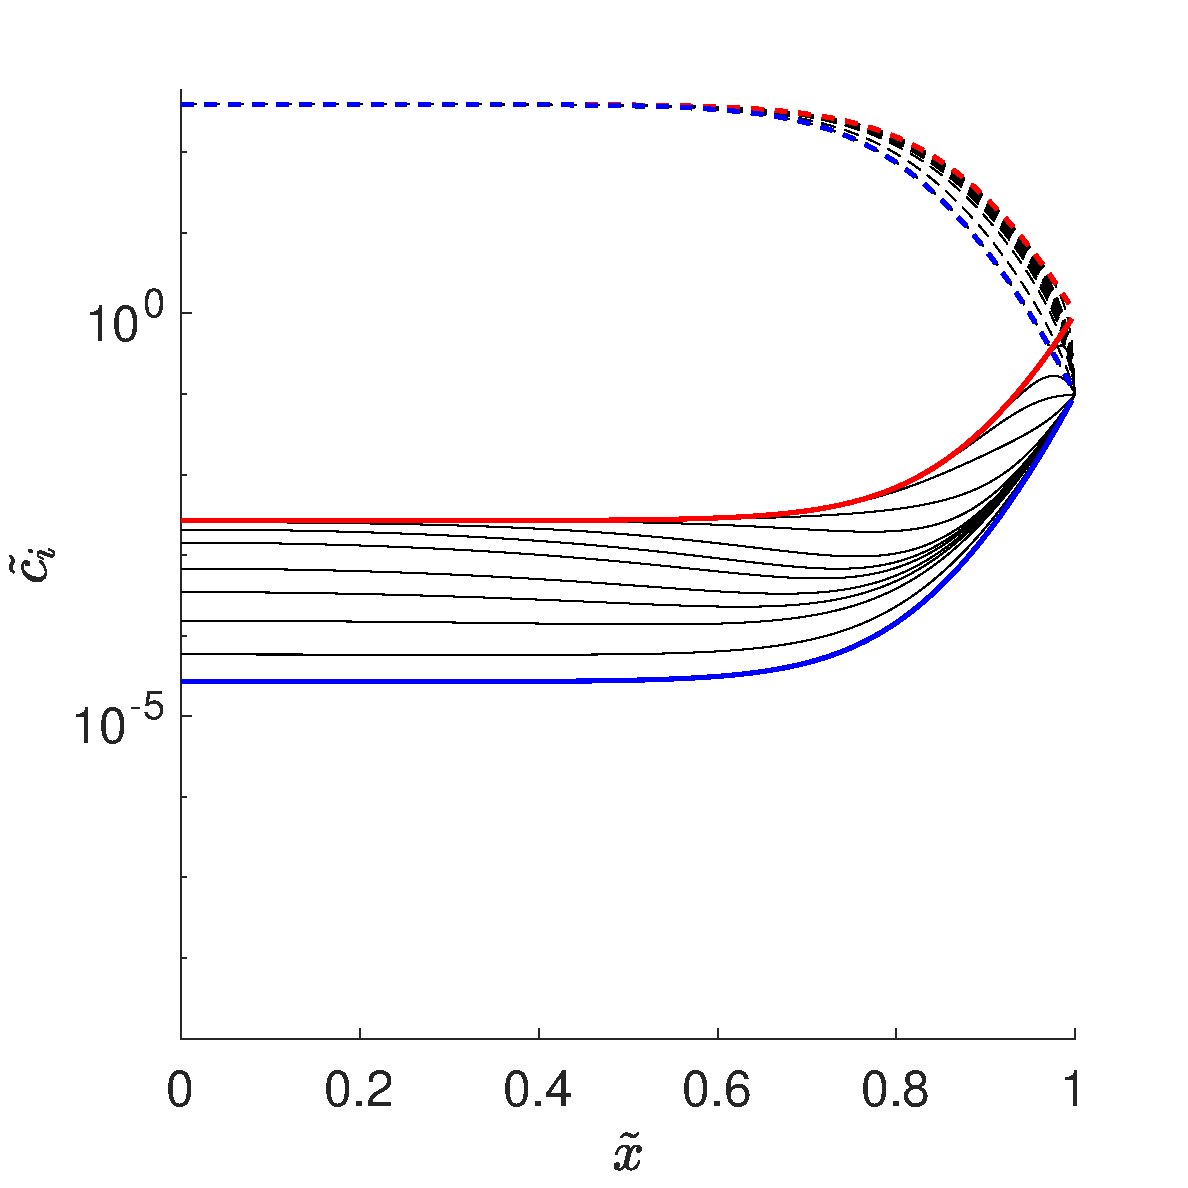
\includegraphics[width=50mm]{narrow_sym/ionProfile_homogeneous.pdf}
	}
	\subfloat[Wide, 1:1 ion]{
		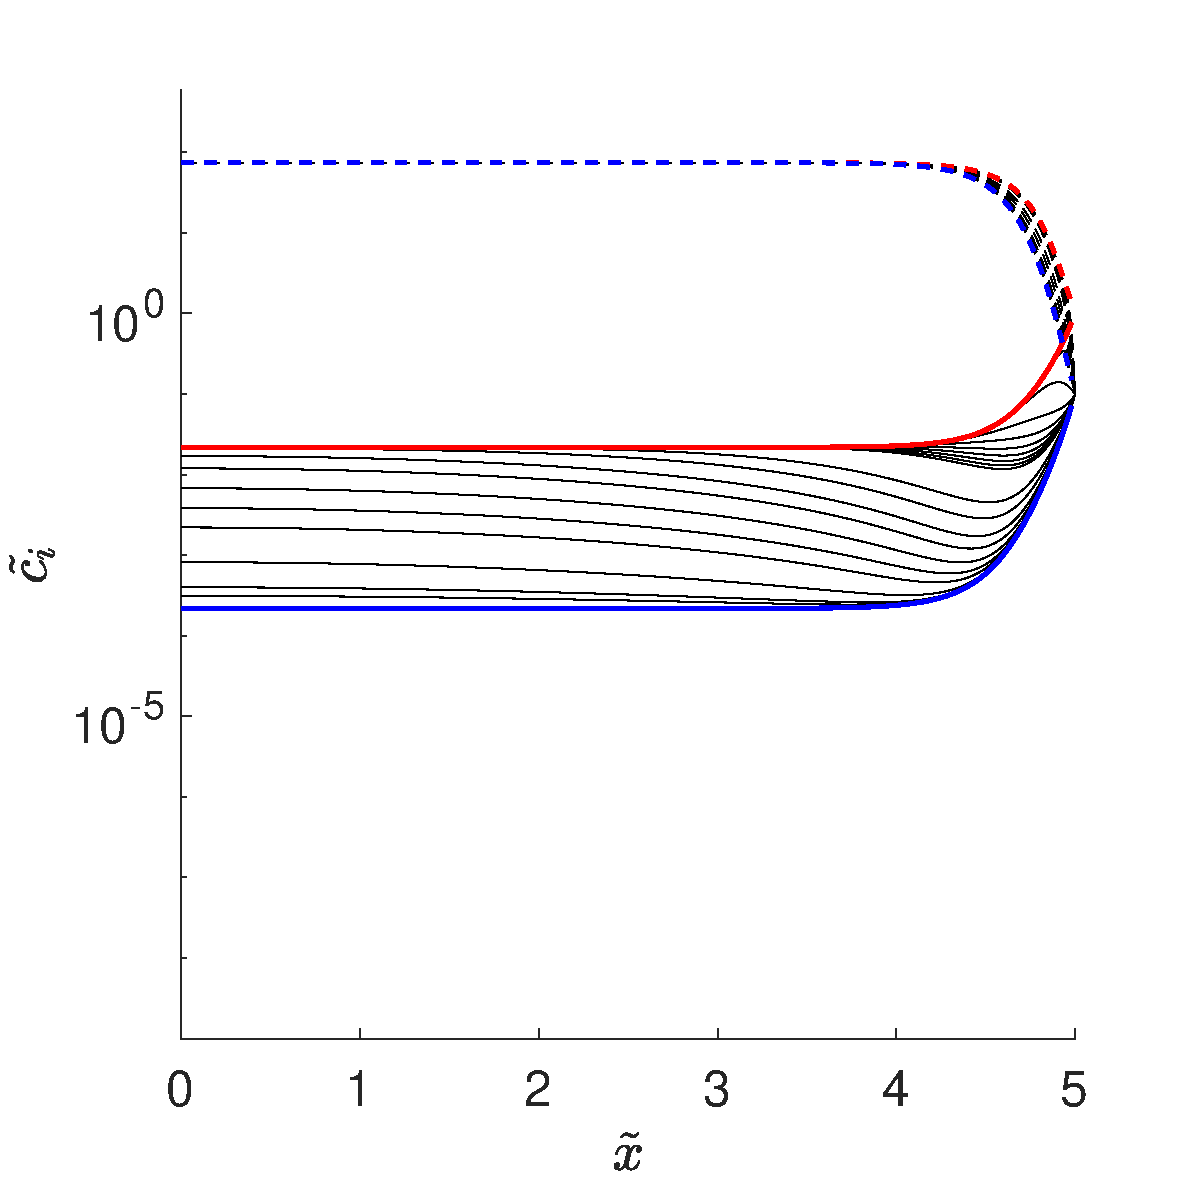
\includegraphics[width=50mm]{wide_sym/ionProfile_homogeneous.pdf}
	}
	\hspace{0mm}
	\subfloat[Narrow, 2:1 ion]{
		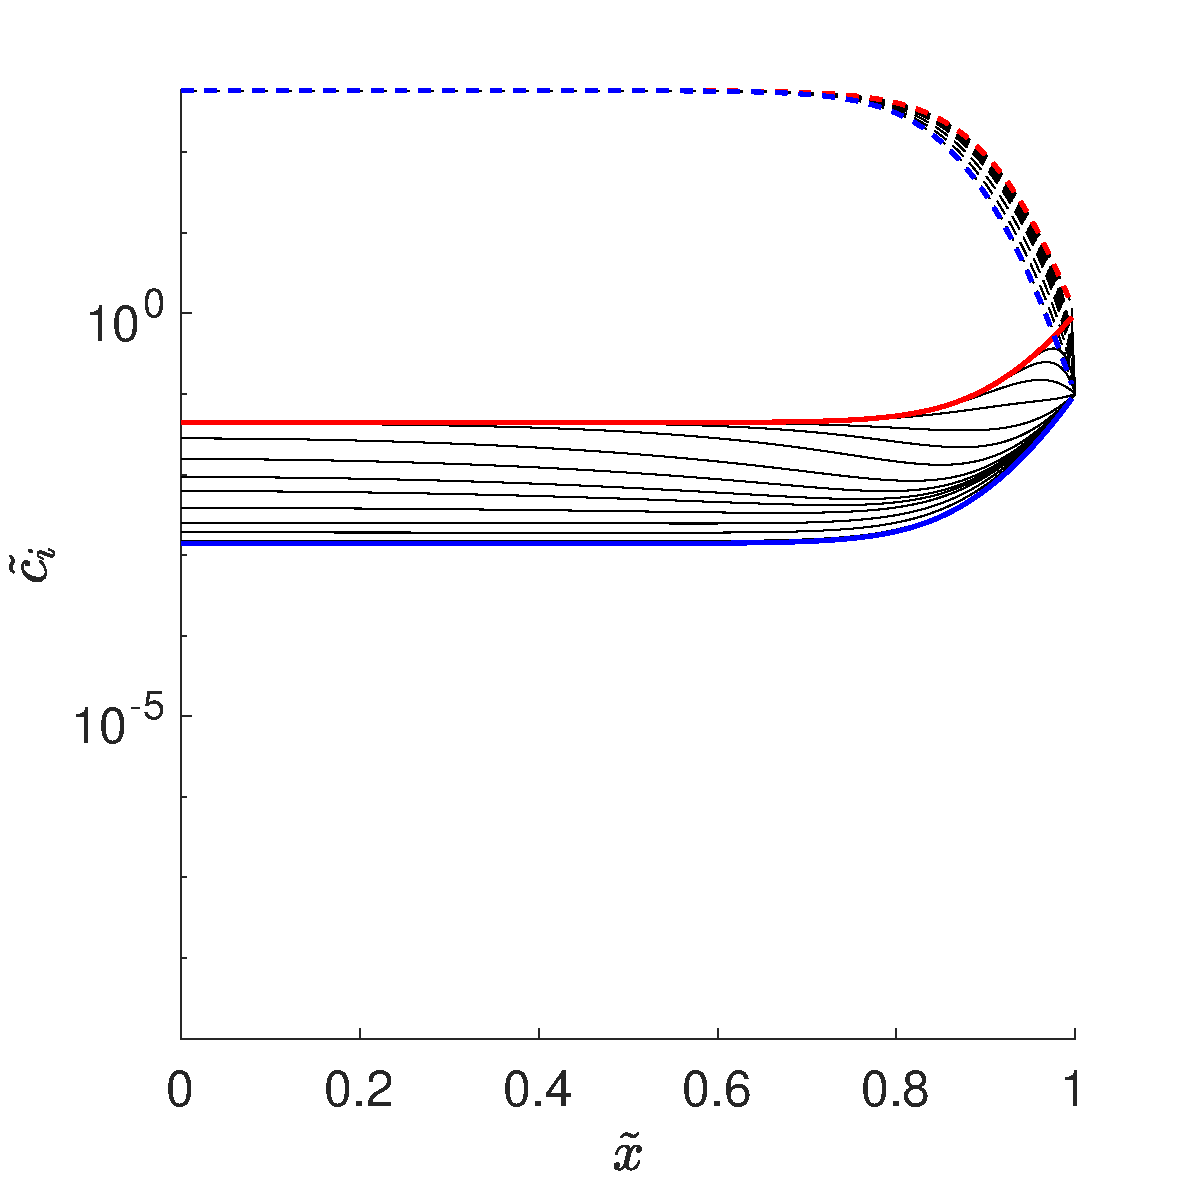
\includegraphics[width=50mm]{narrow_asym_equiIonS/ionProfile_homogeneous.pdf}
	}
	\subfloat[Wide, 2:1 ion]{
		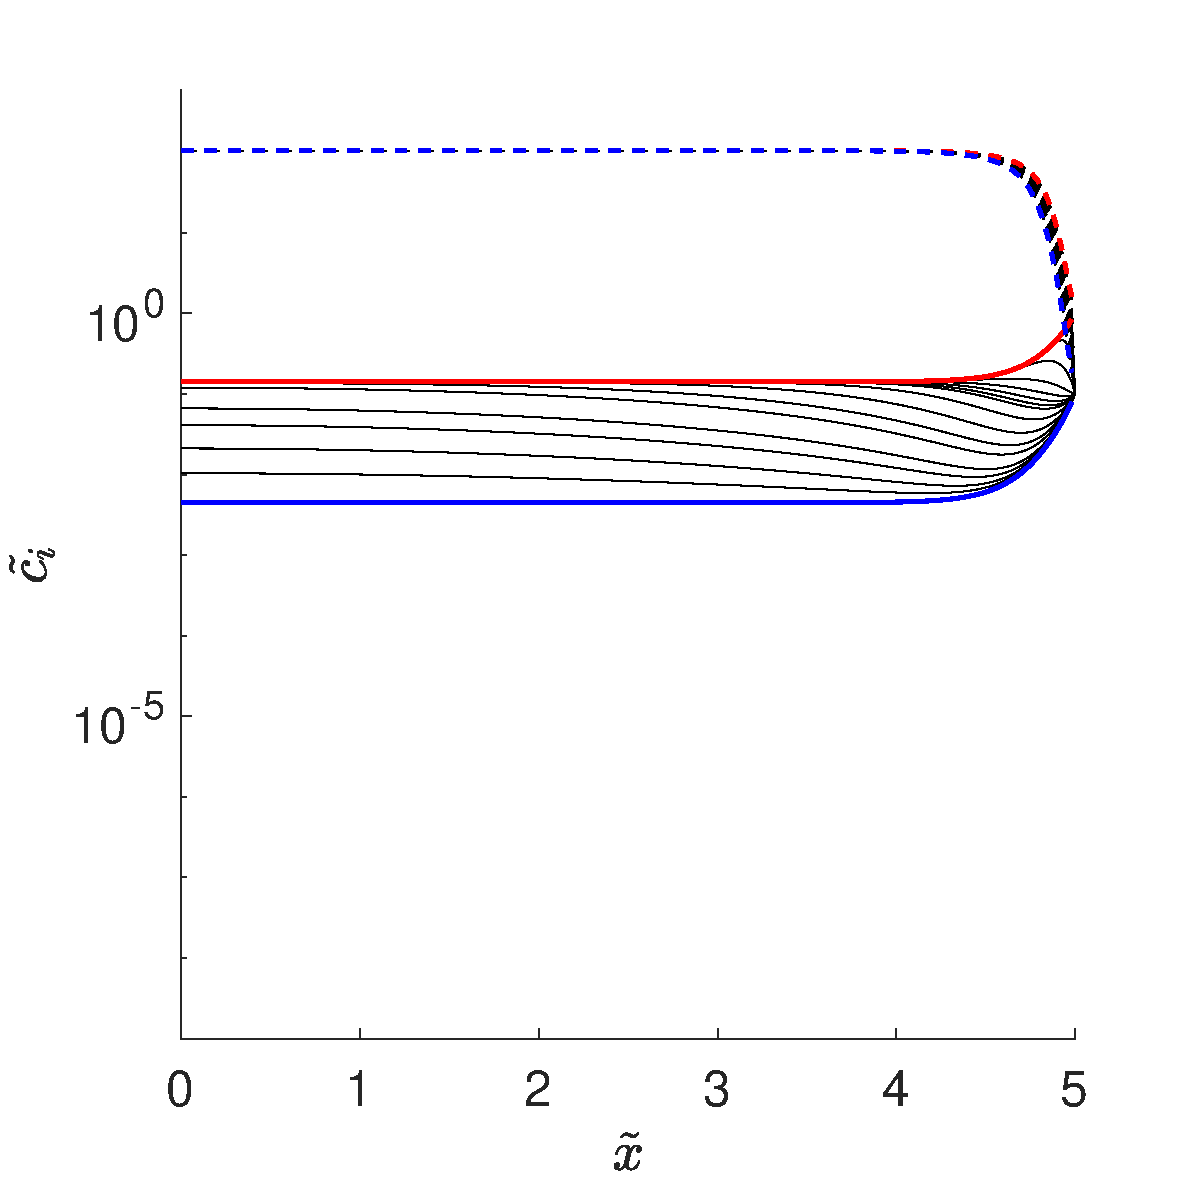
\includegraphics[width=50mm]{wide_asym_equiIonS/ionProfile_homogeneous.pdf}
	}
	\hspace{0mm}
	\subfloat[Narrow, 1:2 ion]{
		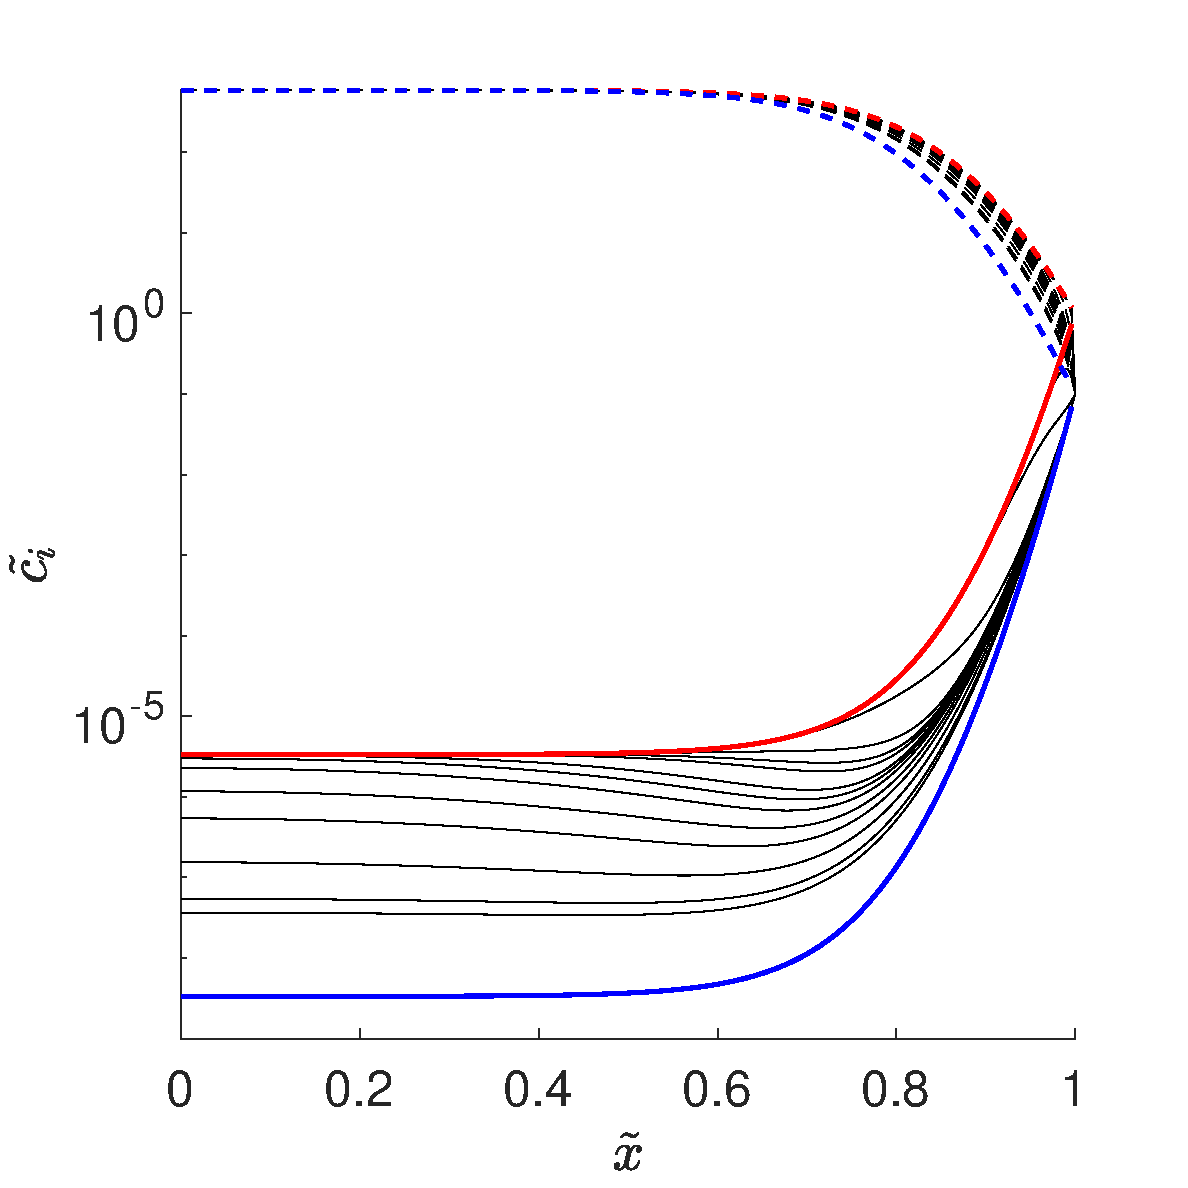
\includegraphics[width=50mm]{narrow_asym_eqIon_inverted/ionProfile_homogeneous.pdf}
	}
	\subfloat[Wide, 1:2 ion]{
		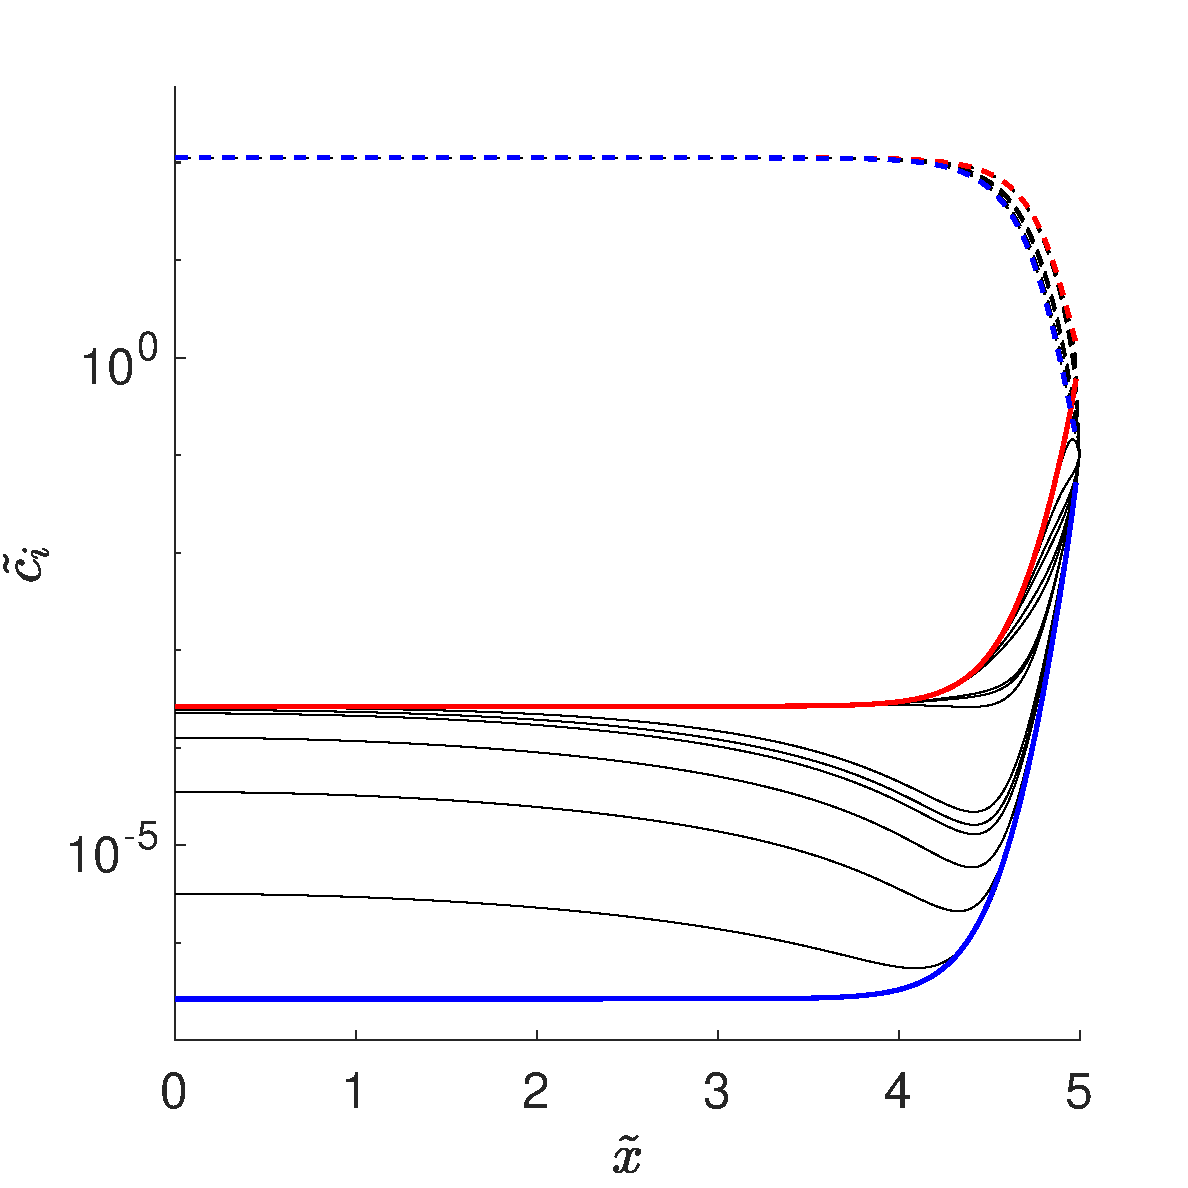
\includegraphics[width=50mm]{wide_asym_eqIon_inverted/ionProfile_homogeneous.pdf}
	}
\label{ionProfiles}
\end{figure}

\newpage

\begin{figure}
	\centering
	\subfloat[Narrow , 1:1 ion]{
		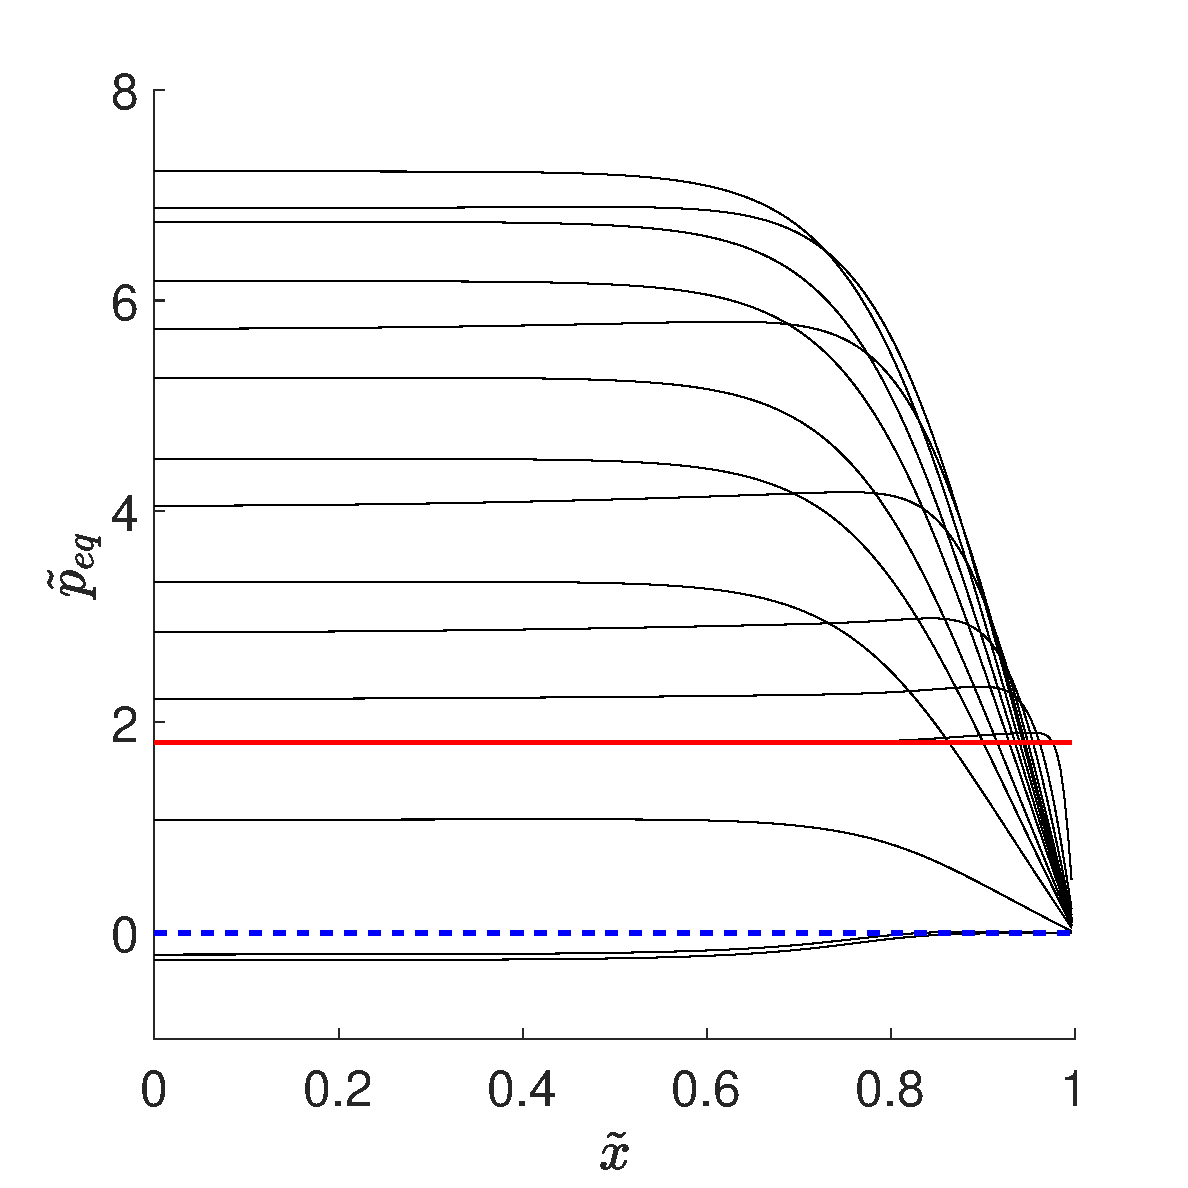
\includegraphics[width=60mm]{narrow_sym/P_ss_homogeneous.pdf}
	}
	\subfloat[Wide , 1:1 ion]{
		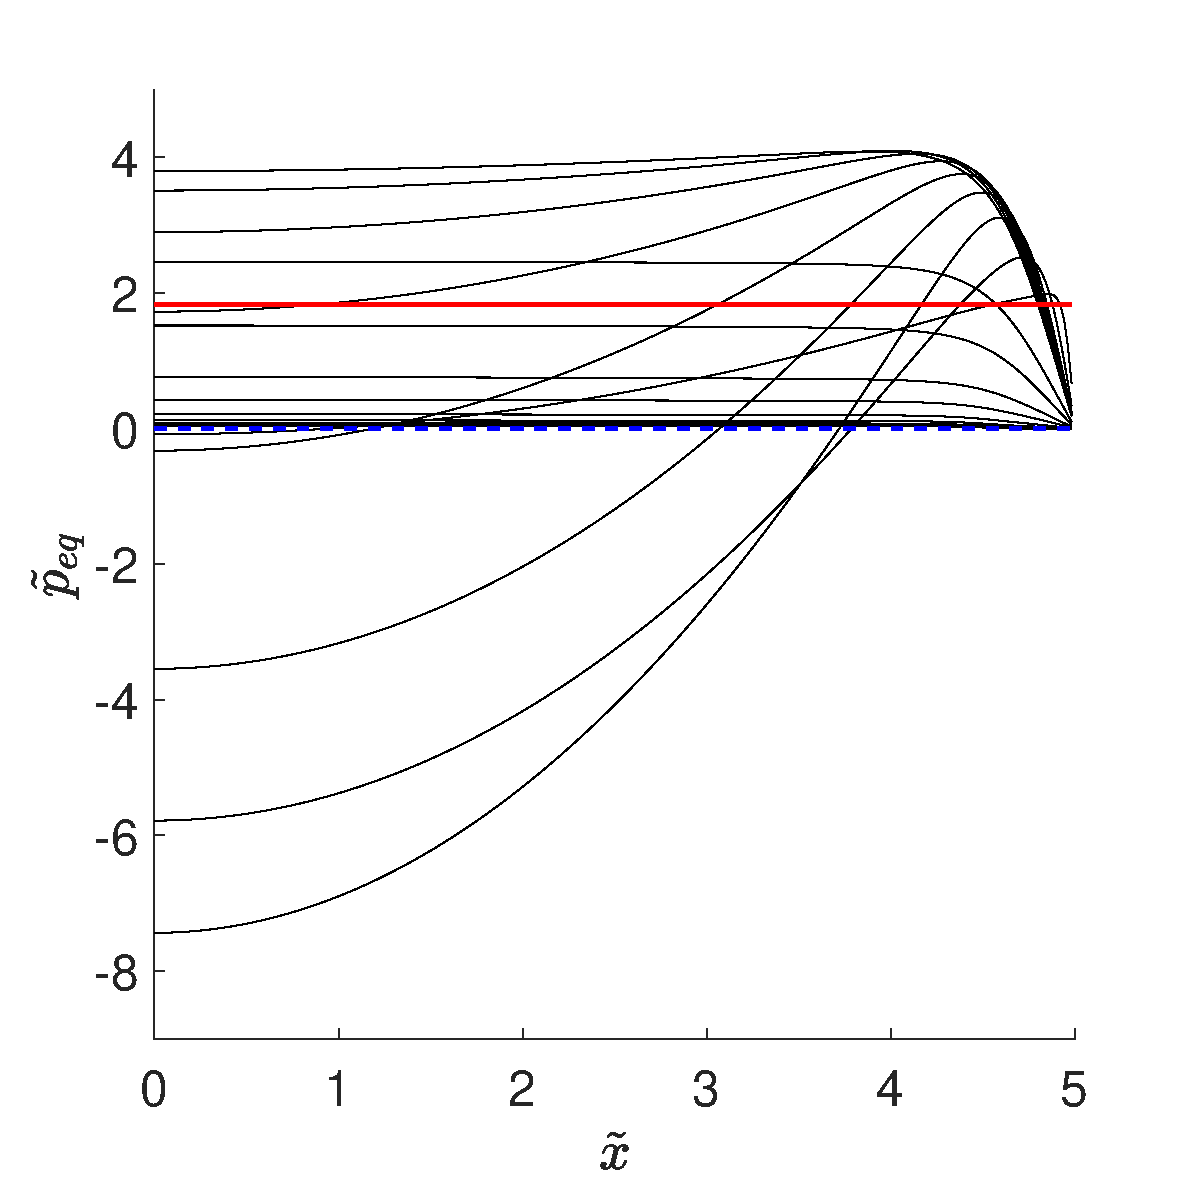
\includegraphics[width=60mm]{wide_sym/P_ss_homogeneous.pdf}
	}
	\hspace{0mm}
	\subfloat[Narrow , 2:1 ion]{
		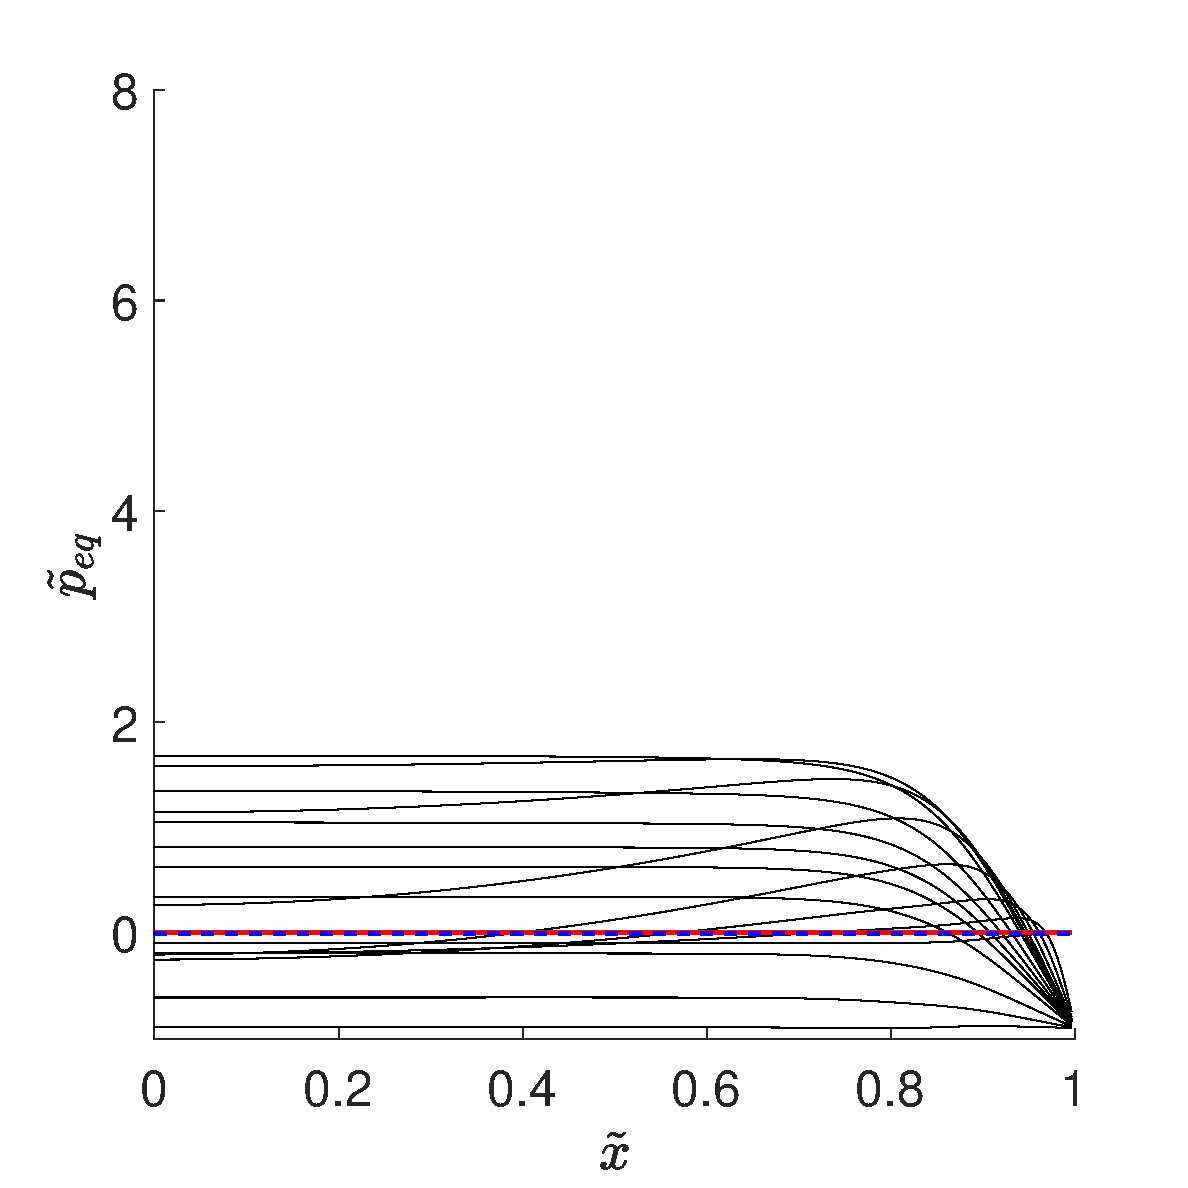
\includegraphics[width=60mm]{narrow_asym_equiIonS/P_ss_homogeneous.pdf}
	}
	\subfloat[Wide , 2:1 ion]{
		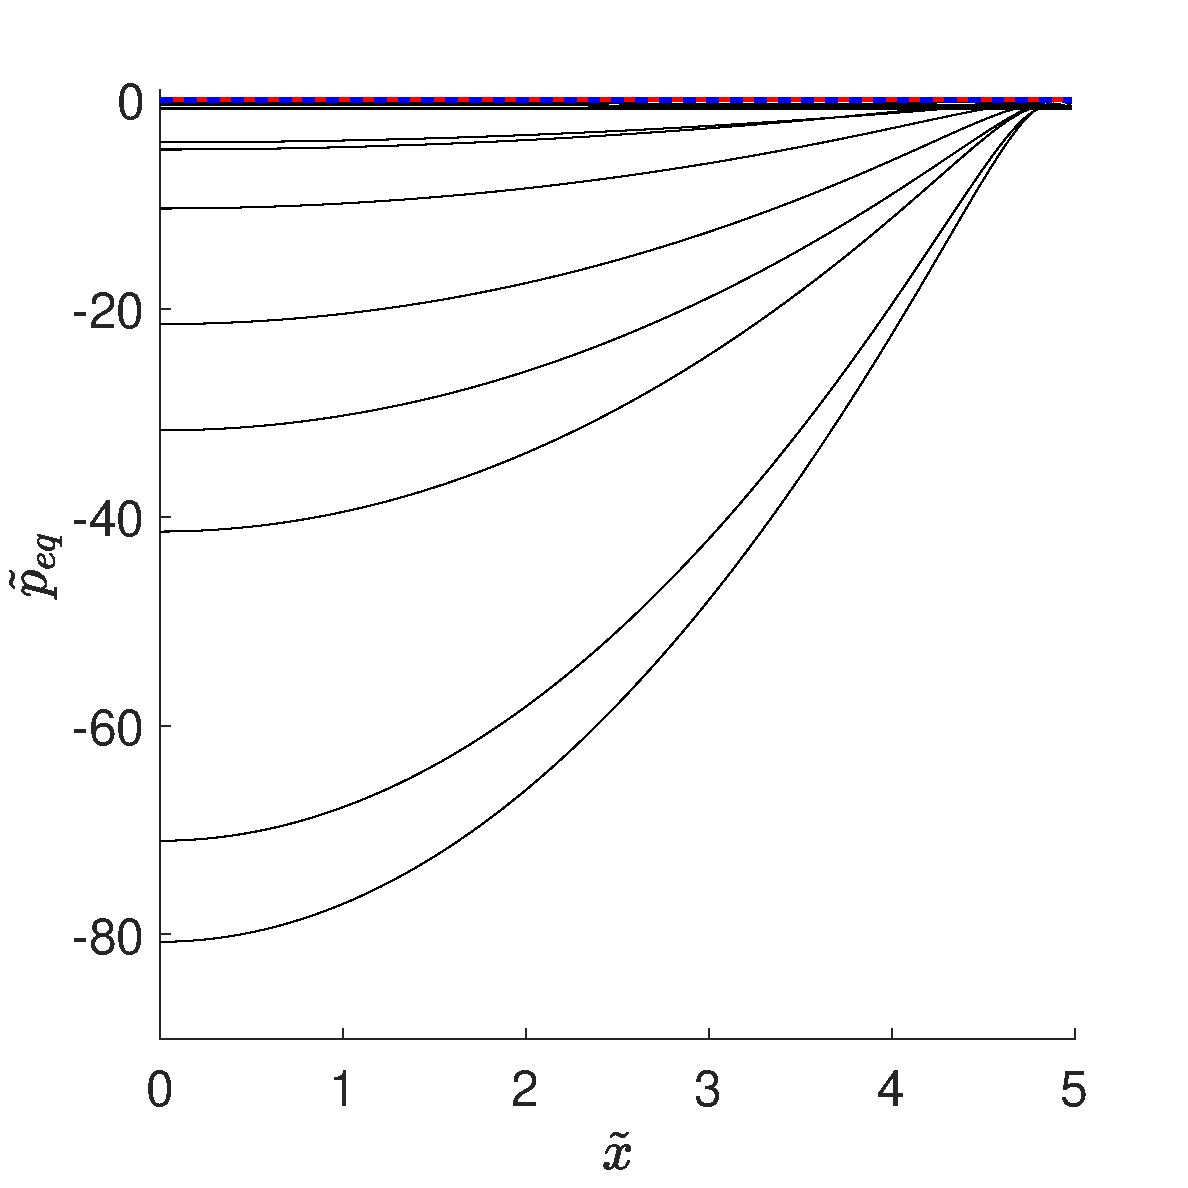
\includegraphics[width=60mm]{wide_asym_equiIonS/P_ss_homogeneous.pdf}
	}
	\hspace{0mm}
	\subfloat[Narrow , 1:2 ion]{
		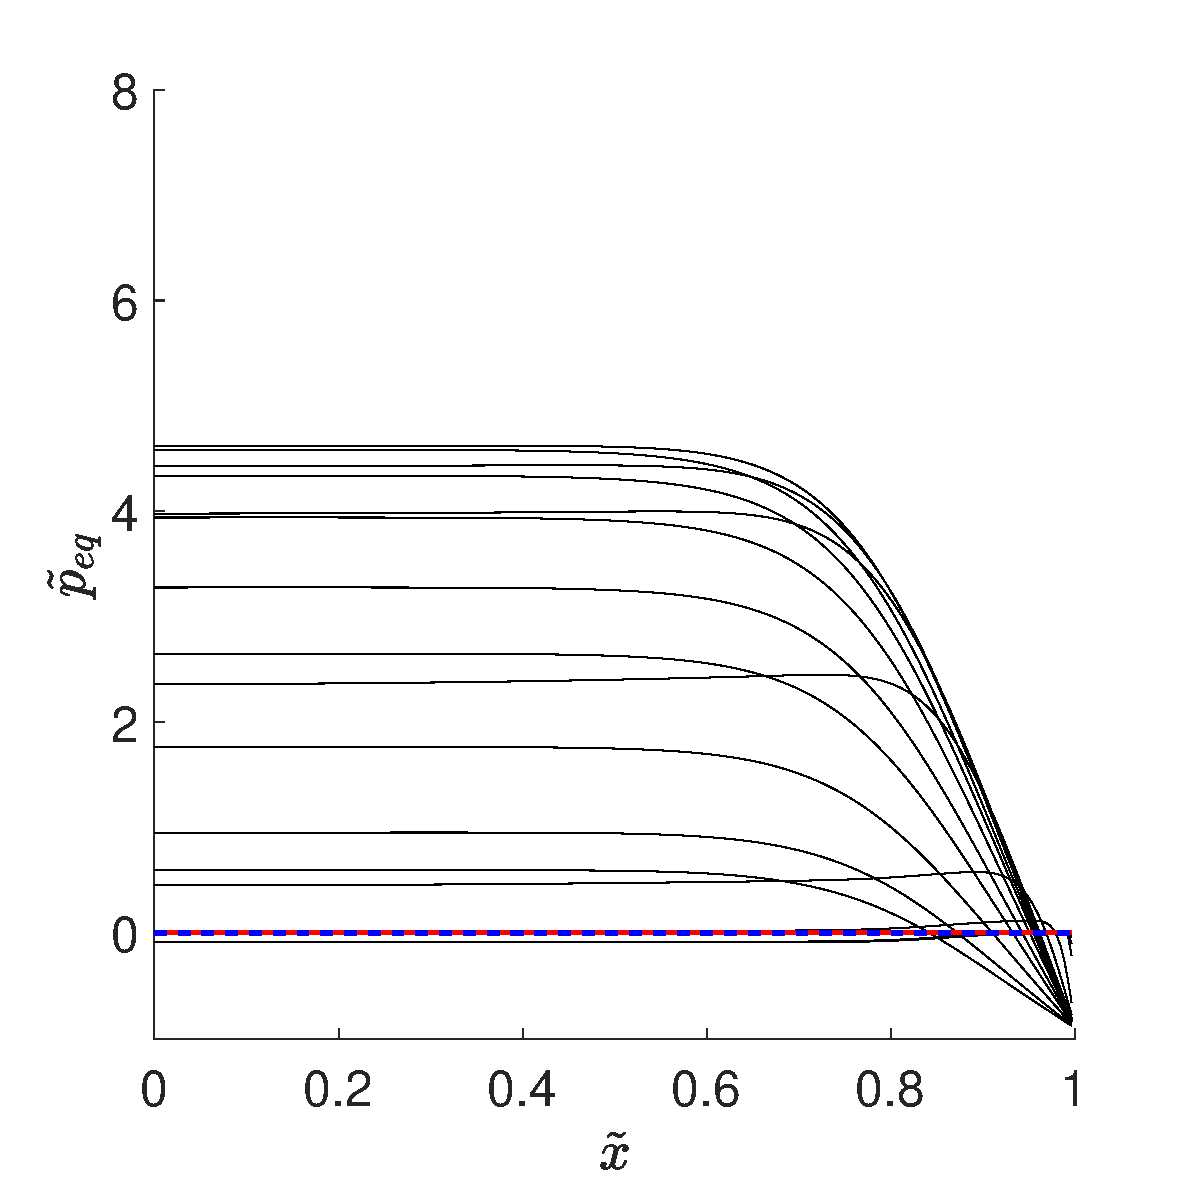
\includegraphics[width=60mm]{narrow_asym_eqIon_inverted/P_ss_homogeneous.pdf}
	}
	\subfloat[Wide , 1:2 ion]{
		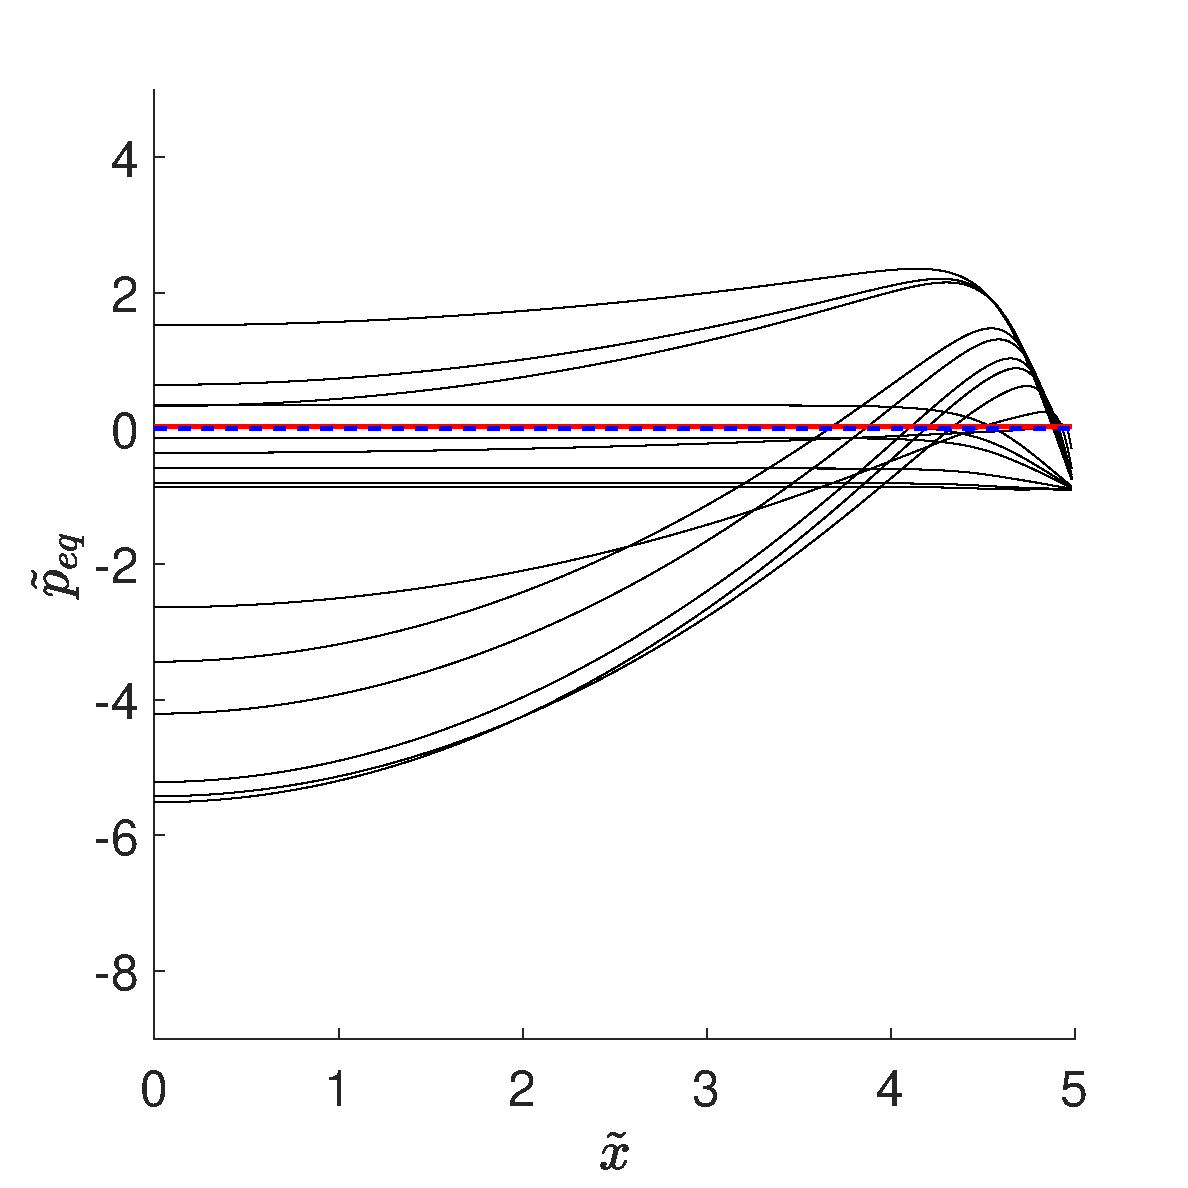
\includegraphics[width=60mm]{wide_asym_eqIon_inverted/P_ss_homogeneous.pdf}
	}
  \label{pressure_eq}
\end{figure}


\begin{comment}
\begin{figure}
	\centering
	\subfloat[Narrow , 1:1 ion]{
		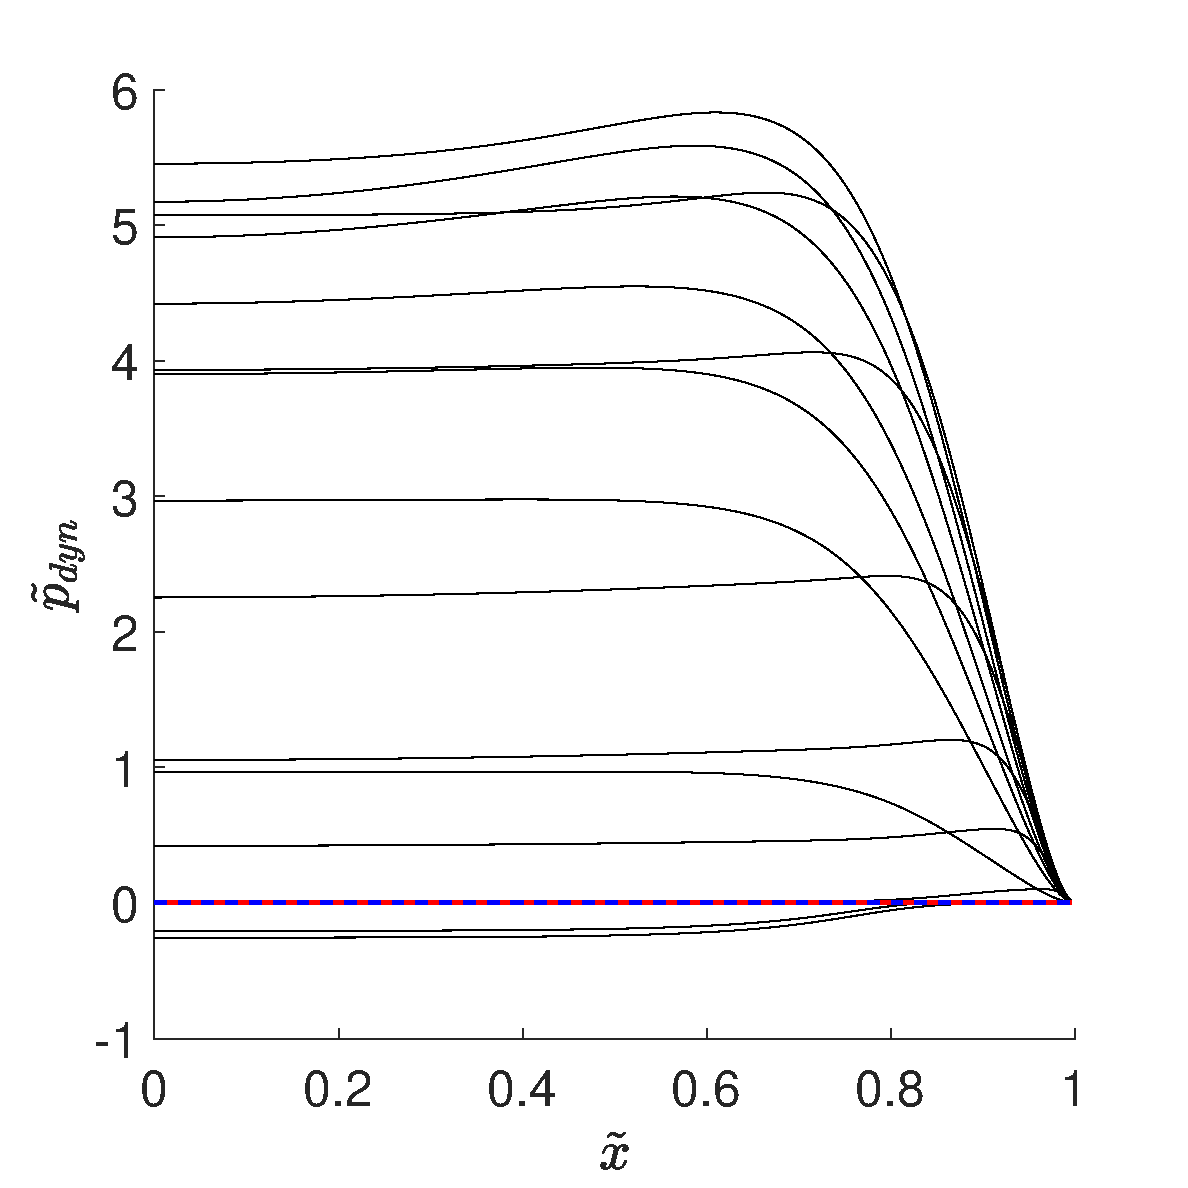
\includegraphics[width=60mm]{narrow_sym/P_dyn_homogeneous.pdf}
	}
	\subfloat[Wide , 1:1 ion]{
		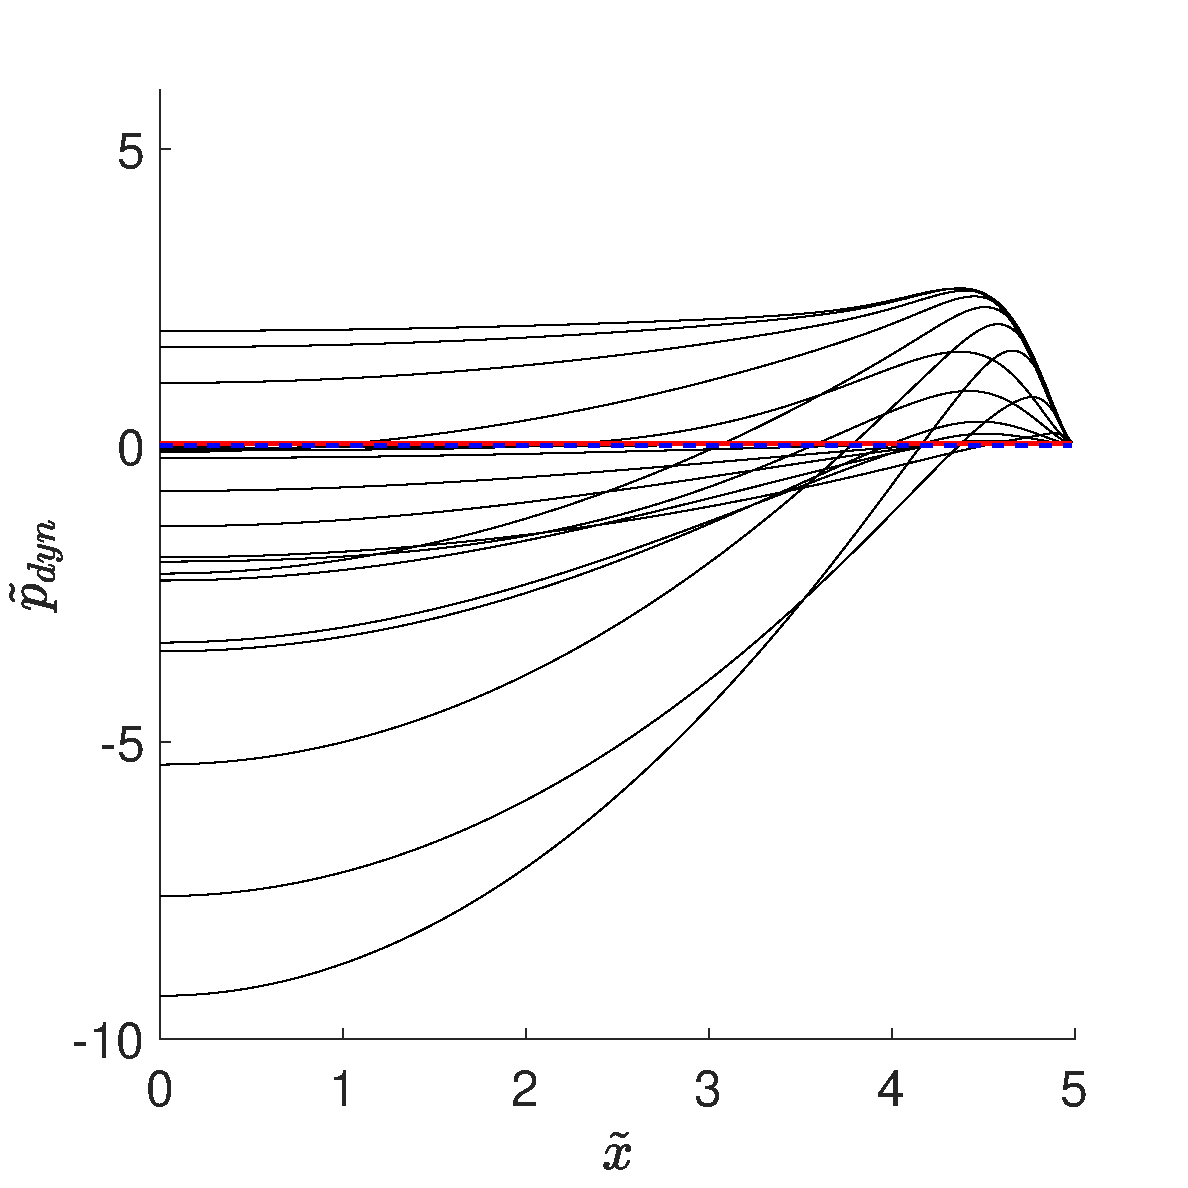
\includegraphics[width=60mm]{wide_sym/P_dyn_homogeneous.pdf}
	}
	\hspace{0mm}
	\subfloat[Narrow , 2:1 ion]{
		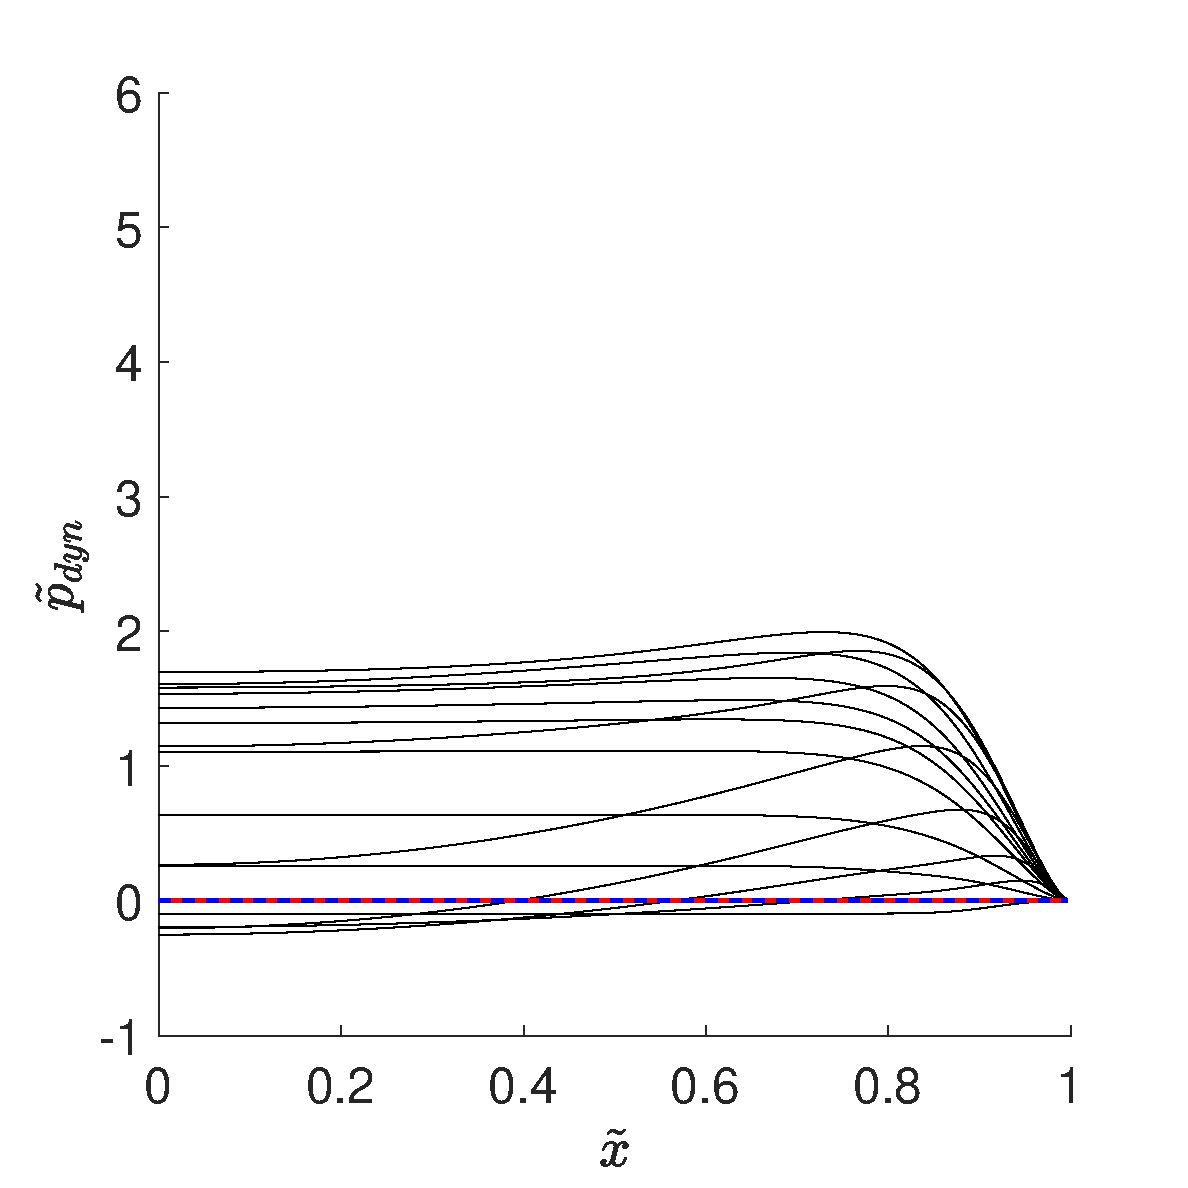
\includegraphics[width=60mm]{narrow_asym_equiIonS/P_dyn_homogeneous.pdf}
	}
	\subfloat[Wide , 2:1 ion]{
		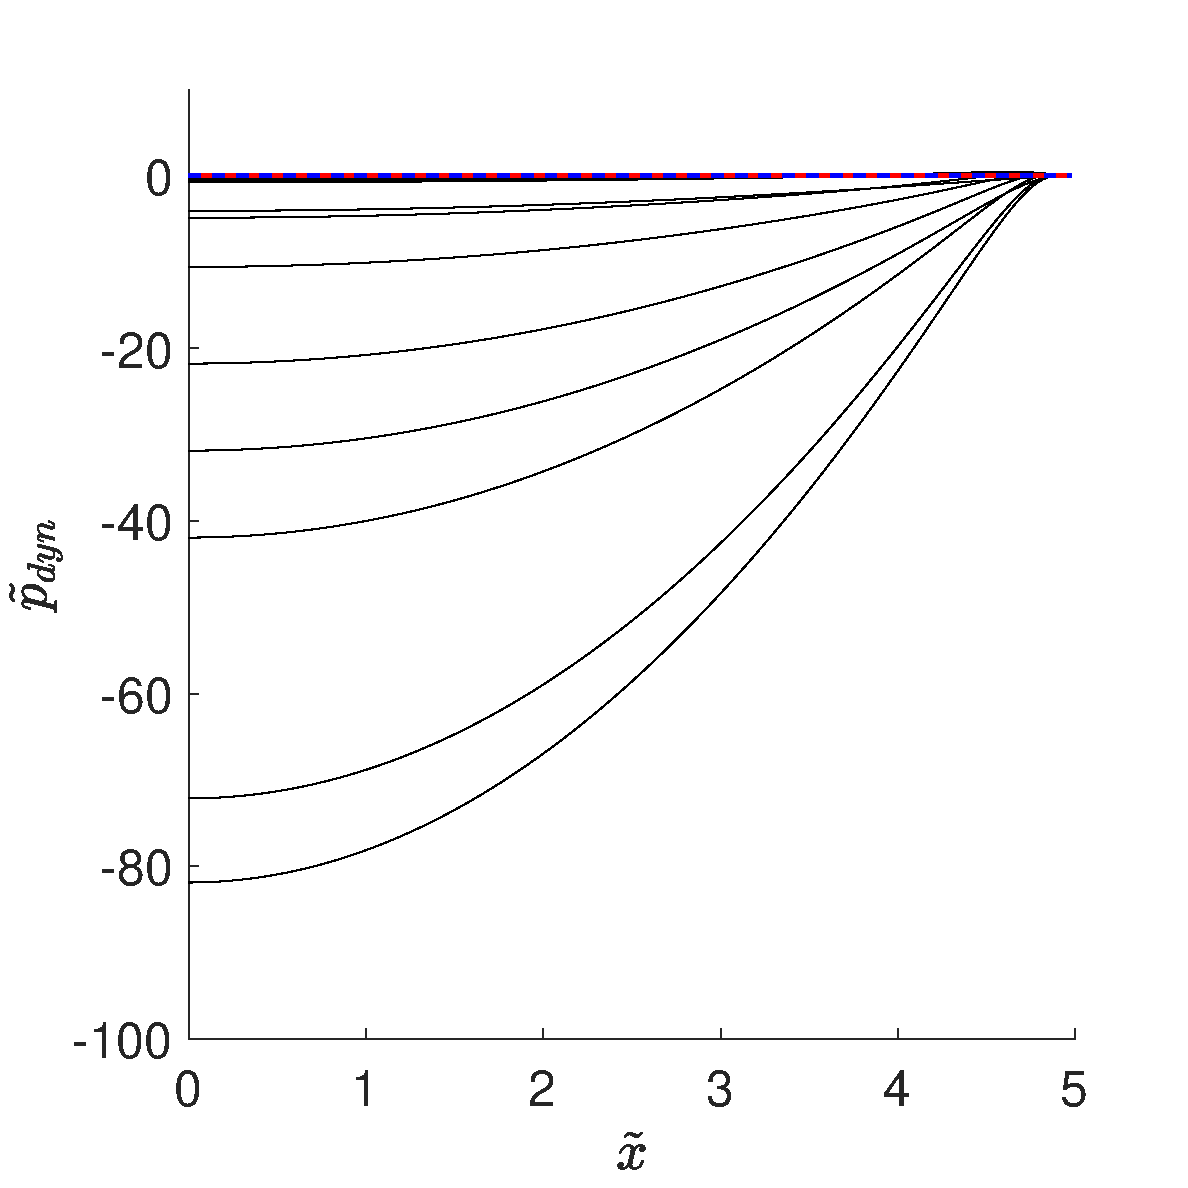
\includegraphics[width=60mm]{wide_asym_equiIonS/P_dyn_homogeneous.pdf}
	}
		\hspace{0mm}
	\subfloat[Narrow , 1:2 ion]{
		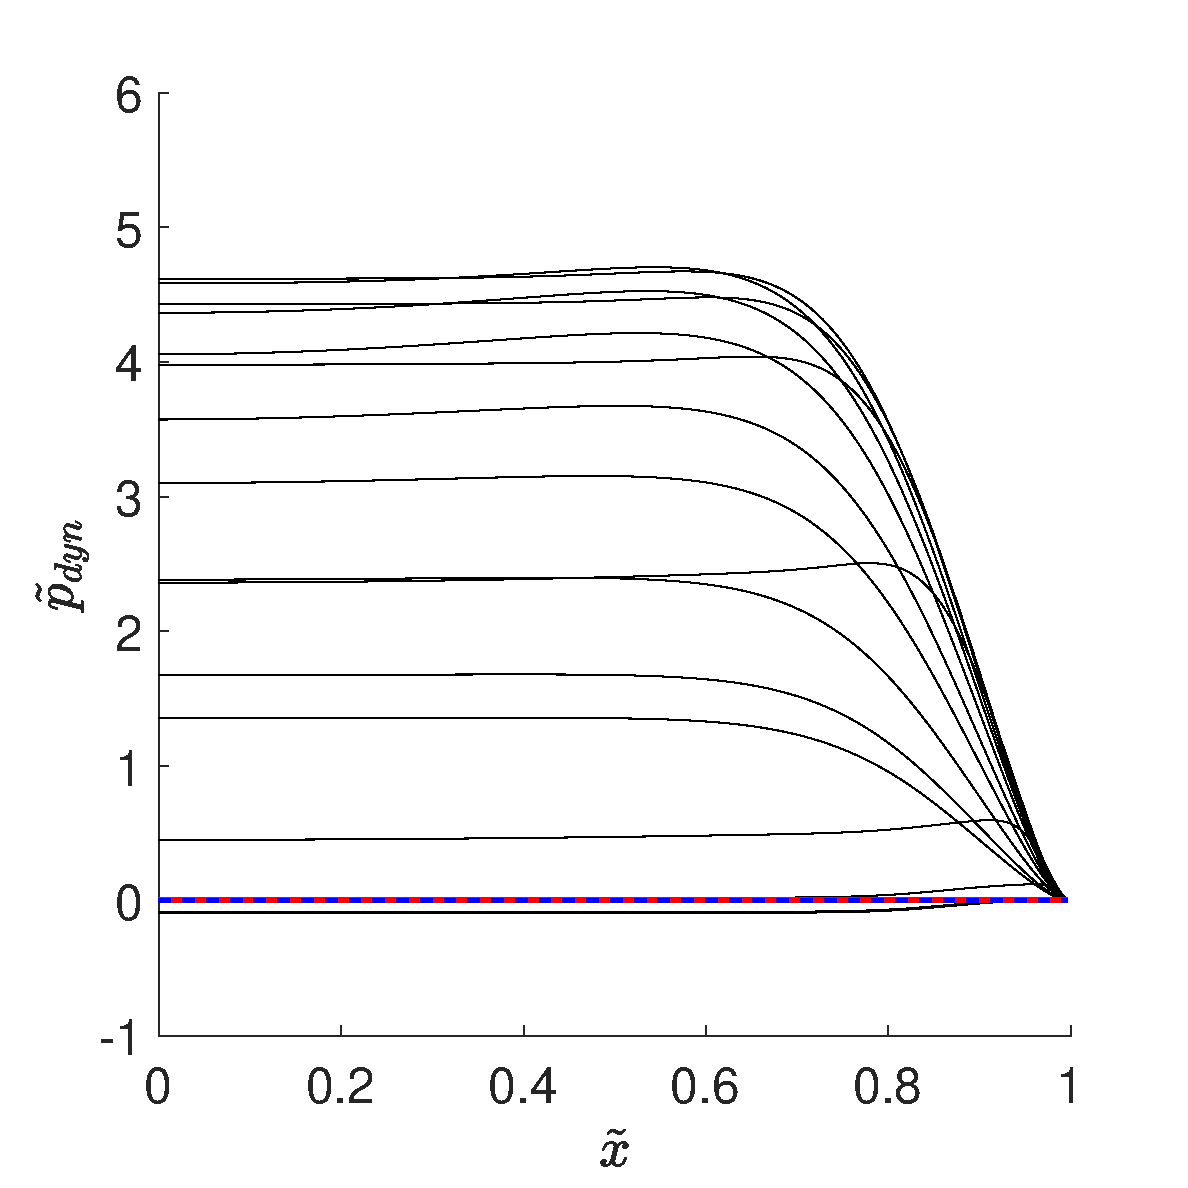
\includegraphics[width=60mm]{narrow_asym_eqIon_inverted/P_dyn_homogeneous.pdf}
	}
	\subfloat[Wide , 1:2 ion]{
		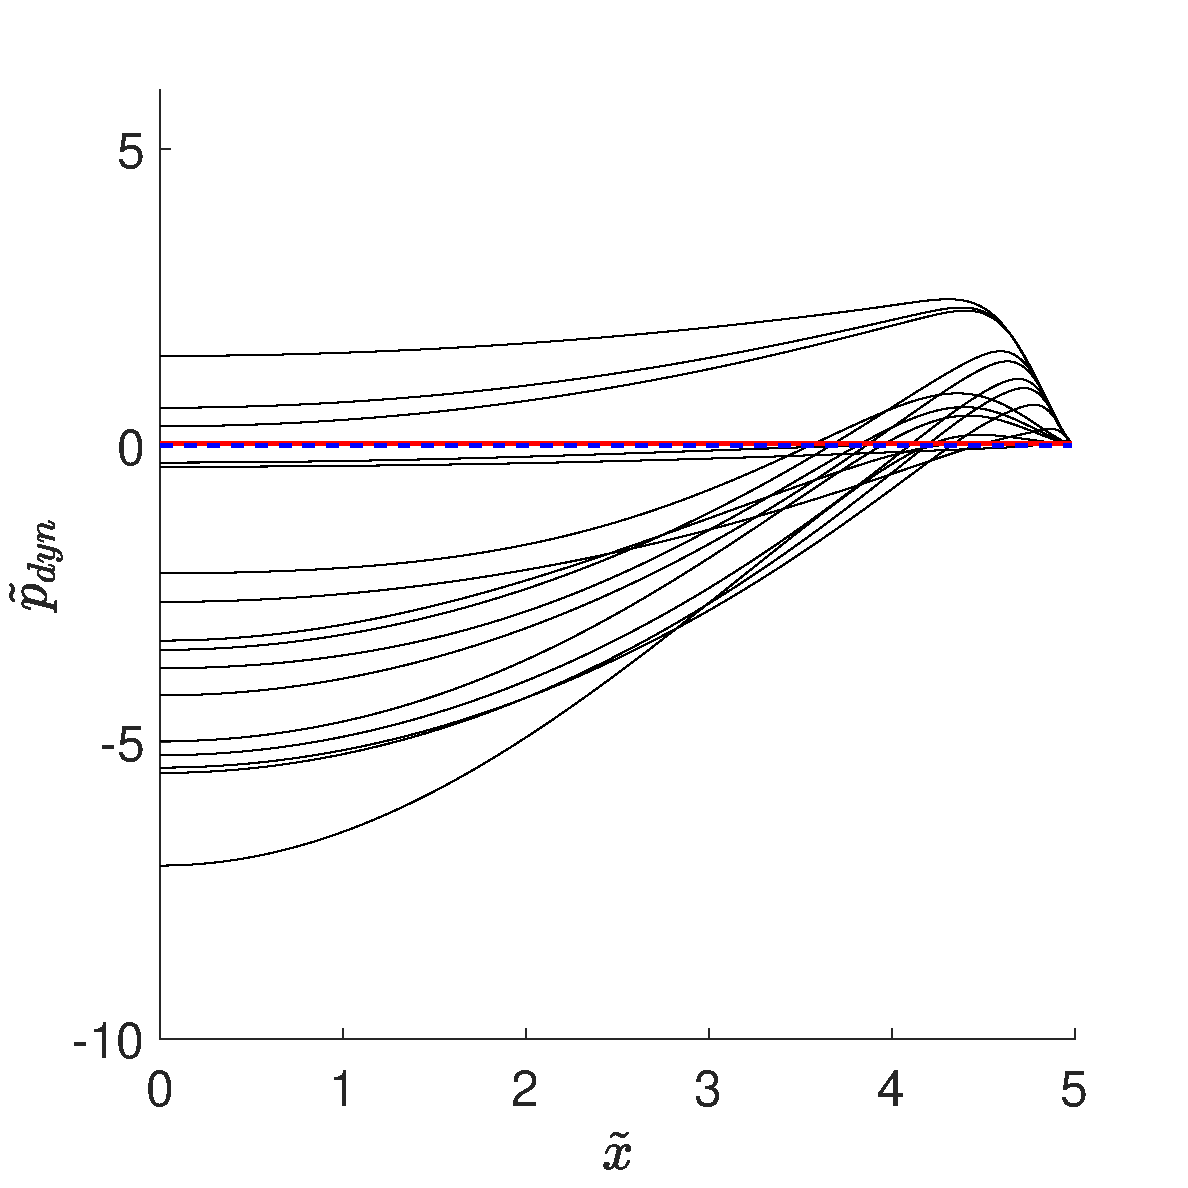
\includegraphics[width=60mm]{wide_asym_eqIon_inverted/P_dyn_homogeneous.pdf}
	}
  \label{pressure_dyn}
\end{figure}

\end{comment}










\end{document}
